\subsection{Privatization}
As with the openOMP version we privatize the \emph{strike} variable. Same
argumentation as before applies.
\textbf{Add more juicy? Do we privatize more? Explain concept and safety? Collapse with the subsection below?}

\subsection{Hoisting of constant values}
\textbf{bad naming of subsection?}
Initializing \emph{globs} allocates the required memory for the variables
\emph{myX}, \emph{myDxx}, \emph{myY}, \emph{myDyy}, \emph{myTimeline},
\emph{myVarX} \& \emph{myVarY}. Since no cross iteration dependecies exist we
can reuse the allocated memory space inbetween each iteration and hoist
\emph{globs} out of the loops. Note that this is a reversal of a privatization,
and could be nonbeneficial, however as \emph{myTimeline}, \emph{myXindex},
\emph{myX}, \emph{myYindex}, \emph{myY}, \emph{Dxx} \& \emph{Dyy} are all
constant accross all iterations and therefore these only need to be computed
once for all iterations. Hence we hoist the \textbf{initGrid} and
\textbf{initOperator} out of the loop as we can see in Figure
\ref{fig:globsinit}.

\begin{figure}[!ht]
\centering
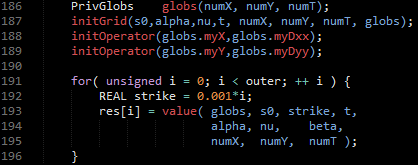
\includegraphics[scale=1]{input/figures/globsinit.png}
\caption{\emph{initGrid} and \emph{initOperator} hoised out of the loop nest.\label{fig:globsinit}}
\end{figure}
 
It it clear that this is a safe code transformation, as these variables are
never written to after they have been initialized.
